\documentclass{article}

\usepackage{tikzStickFigure}

\begin{document}

This is a test to see if the package style file is working as planned.

\vspace{4\baselineskip}

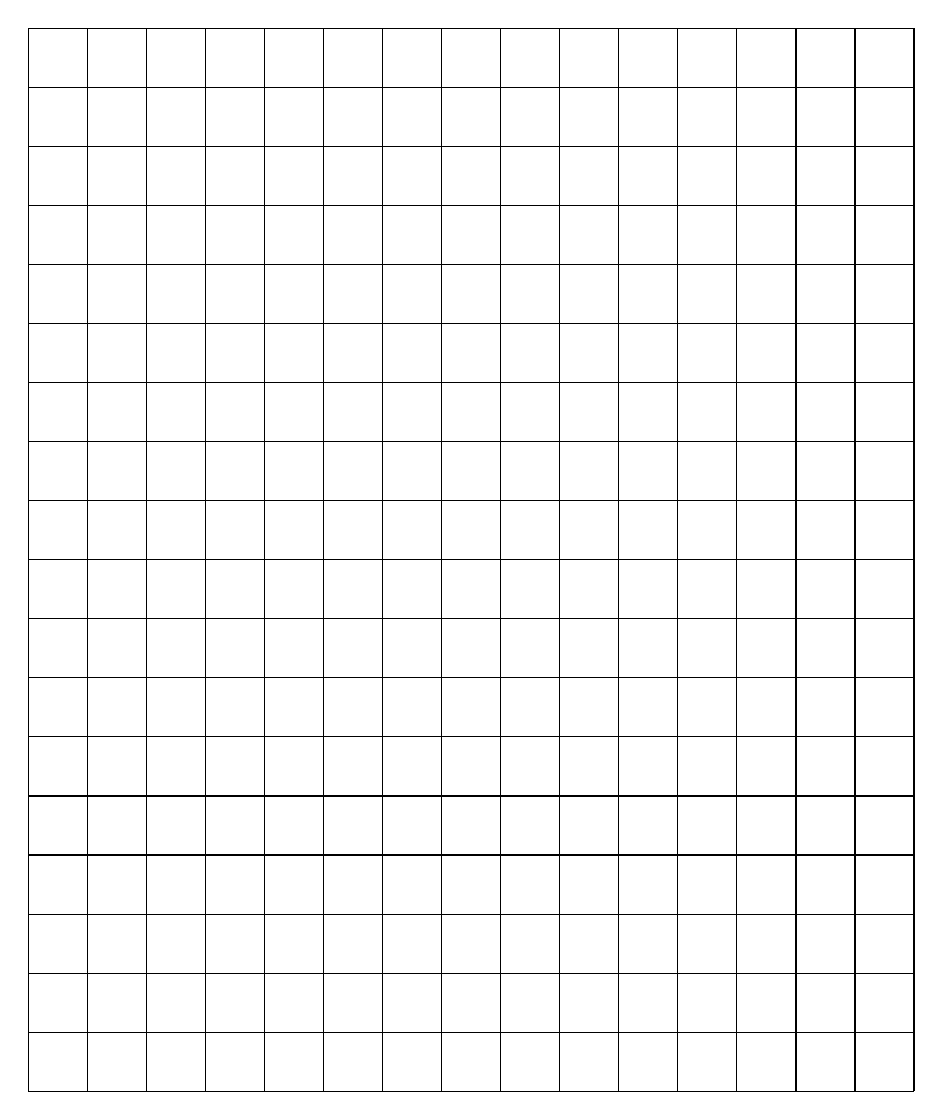
\begin{tikzpicture}[scale=0.75,transform shape]
%% Basic stick figure with nose at (0,0)
    \stickfig

%% Unnamed stick figure 
    \stickfig[stance={run right},position={(1,5)},protection=shield];

%% Named stick figure
    \stickfig[stance=run left,position={(5,-3)},name=chuck,hat=wizard,scale=0.75,weapon=sword];
    
    
    \draw (-5,-10) grid (10,8);

\end{tikzpicture}


\end{document}
